\documentclass[12pt,utf8, handout]{beamer}
\setbeamercovered{transparent}
\usepackage[german]{babel}
\usepackage{color}
\usepackage{xcolor}
\usepackage{graphicx}
\usepackage{tikz}
%\usetheme{Latex_Template/beamerthemeFOSSAG.sty}
\input{design_latex-template/beamerthemeFOSSAG.sty}

\title{Threads vs. Multiprocessing}
\subtitle{Ain't nobody got time for dat}

\author{ThiefOfTime}
\institute[FOSS AG]{
\includegraphics[height=0.3\textheight]{img/logo_text-voll-transp.png}}


\date{\today}

\begin{document}

\begin{frame}

\titlepage

\end{frame}

\begin{frame}
\frametitle{Worum geht es?}
\begin{itemize}
	\item Was sind Threads?
	\item Wie funktionieren Threads in Python?
	\item Wie funktioniert Multiprocessing in Python?
	\item Vergleich von normaler Ausführung, Threads und Multiprocessing
	\item Einsatzgebiete von Threads und Multiprocessing
\end{itemize}
\end{frame}

\begin{frame}
\frametitle{Threads - Generell}
\begin{figure}
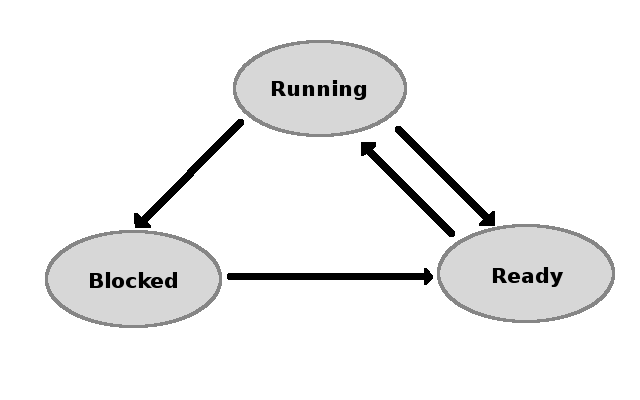
\includegraphics[scale=0.25]{img/thread.png}
\end{figure}
\begin{itemize}
	\item Threads des selben Prozesses verwenden den gleichen Adressraum
	\item Kommunikation zwischen Threads daher sehr einfach
	\item Jeder Thread führt eine Aufgabe aus
	\item Aufteilen auf mehrere Prozessorkerne möglich
\end{itemize}
\end{frame}

\begin{frame}
\frametitle{Threads - Java}
\begin{figure}

\includegraphics[scale=0.15]{img/serveimage.jpeg}
\end{figure}
\begin{itemize}
	\item Verwaltet Threads durch virtuelle Maschine
	\item Unterstütung von Multithreading selbst auf Systemen, die Multithreading nicht unterstützen
	\item Blockieren den Zugriff auf geteilte Daten
	\item Threads können nicht von außen abgebrochen werden (Deadlocks bzw. Inkonsistenz)
\end{itemize}
\end{frame}

\begin{frame}
\frametitle{Threads in Python}
\begin{itemize}
	\item \texttt{threading} package ist light weight
	\item Teilen des Speichers unter allen Threads
	\item Python interpreter ist nicht Thread sicher
	\item Einsetzen von Global Interpreter Lock
\end{itemize}
\end{frame}

\begin{frame}
\frametitle{GIL - Global Interpreter Lock}
\begin{figure}

\includegraphics[scale=0.2]{img/hydra1.png}
\end{figure}
\begin{itemize}
	\item Verhindern des gleichzeitigen Ausführens von mehreren Threads in einem Python Interpreter
	\item Jeder Thread der laufen will muss auf GIL warten
	\item Byte Code ist der Schlüssel zum befreien
	\item Befreien nach 100 Byte Code Anweisungen durch CPython
\end{itemize}
\end{frame}

\begin{frame}
\frametitle{Multiprocessing in Python}
\begin{figure}

\includegraphics[scale=0.2]{img/hydra.png}
\end{figure}
\begin{itemize}
	\item Ausführen einer Anweisung als eigenständigen Prozess (eigener Speicher und Interpreter)
	\item Stoppen der einzelnen Prozesse möglich
	\item kann evtl in hohem IO Overhead resultieren
\end{itemize}
\end{frame}

\begin{frame}
\frametitle{Vergleich}
Lasst es uns mal an einem Beispiel angucken
\end{frame}

\begin{frame}
\frametitle{Ergebnisse}
\begin{tabular}{l | c | c | c | r}
Art / Anzahl & 2 & 4 & 6 & 8 \\ \hline
Simple & 3.175 & 6.224 & 8.659 & 11.419 \\ \hline
Thread & 4.832 & 11.345 & 18.344 & 24.598 \\ \hline
Processes & 1.334 & 1.630 & 4.181 & 3.228 \\
\end{tabular}
\end{frame}

\begin{frame}
\frametitle{Warum sollte man Threads nutzen?}
\begin{itemize}
	\item Threads sind praktisch für IO-Prozesse (nur auf Bandbreite angewiesen)
	\item Sobald auf geteilte Daten zugegriffen werden
	\item nicht sinnvoll für Berechnungen
\end{itemize}
\end{frame}

\end{document}